\documentclass[11pt]{article}
\usepackage[utf8]{inputenc}
\usepackage[french]{babel}
\usepackage{graphicx}
\usepackage[T1]{fontenc}
%\usepackage{amss}
\usepackage{amsmath}
\usepackage{amsfonts}
\usepackage{amssymb}
\usepackage[left=1.5cm,right=1.5cm,top=1.5cm,bottom=1.5cm]{geometry}

\newcommand\comment{}
\def\N{\mathbb N}
\def\R{\mathbb R}
\def\Q{\mathbb Q}
\def\Z{\mathbb Z}
\begin{document}
\title{\vspace{-2.5cm}PARTIEL I31, Dijon, 2017}
\date{}\maketitle

\section{Problème 1~: dates au plus tôt et au plus tard}

Recopiez ce graphe sur votre feuille d'examen. Indiquez les dates au plus tôt et au plus tard sur les sommets du graphe, 
et soulignez le chemin critique. 

\begin{center}
\includegraphics[width=0.7\linewidth]{critique2.eps}
\end{center}

Quel problème concernant des séquences a été réduit en cours à un problème de
dates au plus tôt et au plus tard~?

Le graphe complété est donné ci-dessous. Le calcul de la plus longue séquence commune à deux séquences données a été réduit en cours à un problème de dates au plus tôt et au plus tard.

\begin{center}
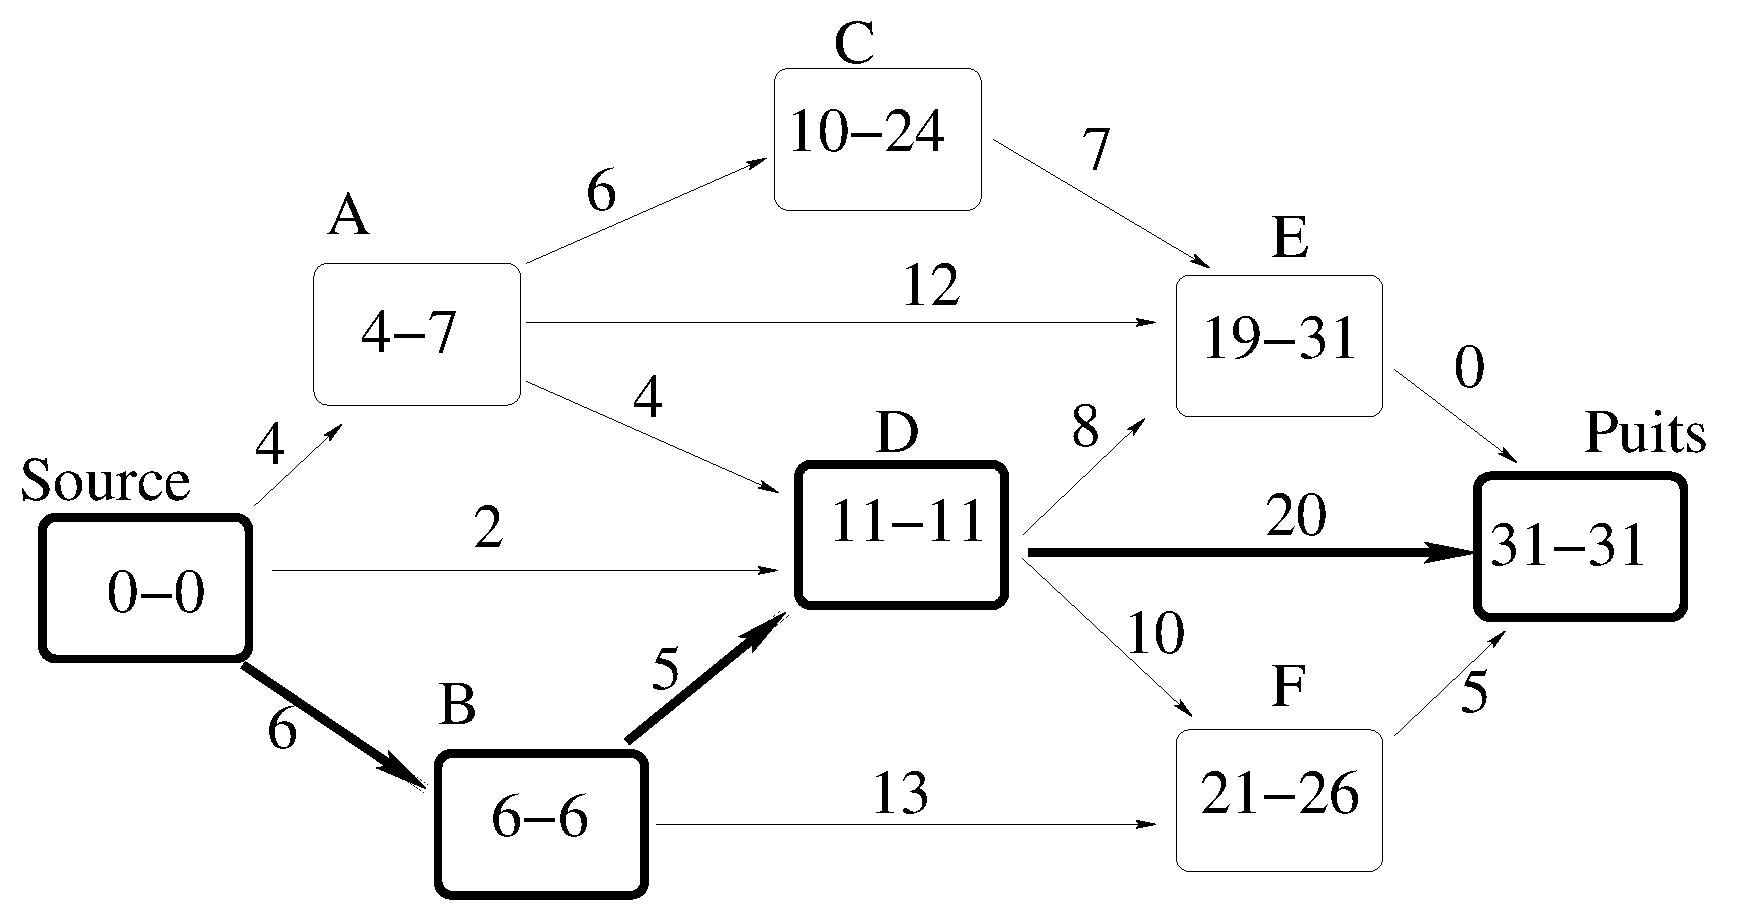
\includegraphics[width=0.75\linewidth]{critique2_solution.eps}
\end{center}


\section{Problème 2~: tri topologique}
Pour redessinez le graphe ci-dessous pour que tous les arcs aillent de gauche à droite (comme ceci~: $\rightarrow$):
Quels sont les premiers sommets possibles~?
Quels sont les derniers sommets possibles~? Pourquoi~?


Redessinez le graphe.

Les premiers sommets possibles sont ceux sans arc entrant (5).
Les derniers sommets possibles sont ceux sans arc sortant (6).

Le graphe redessiné est donné ci-dessous.



\begin{center}
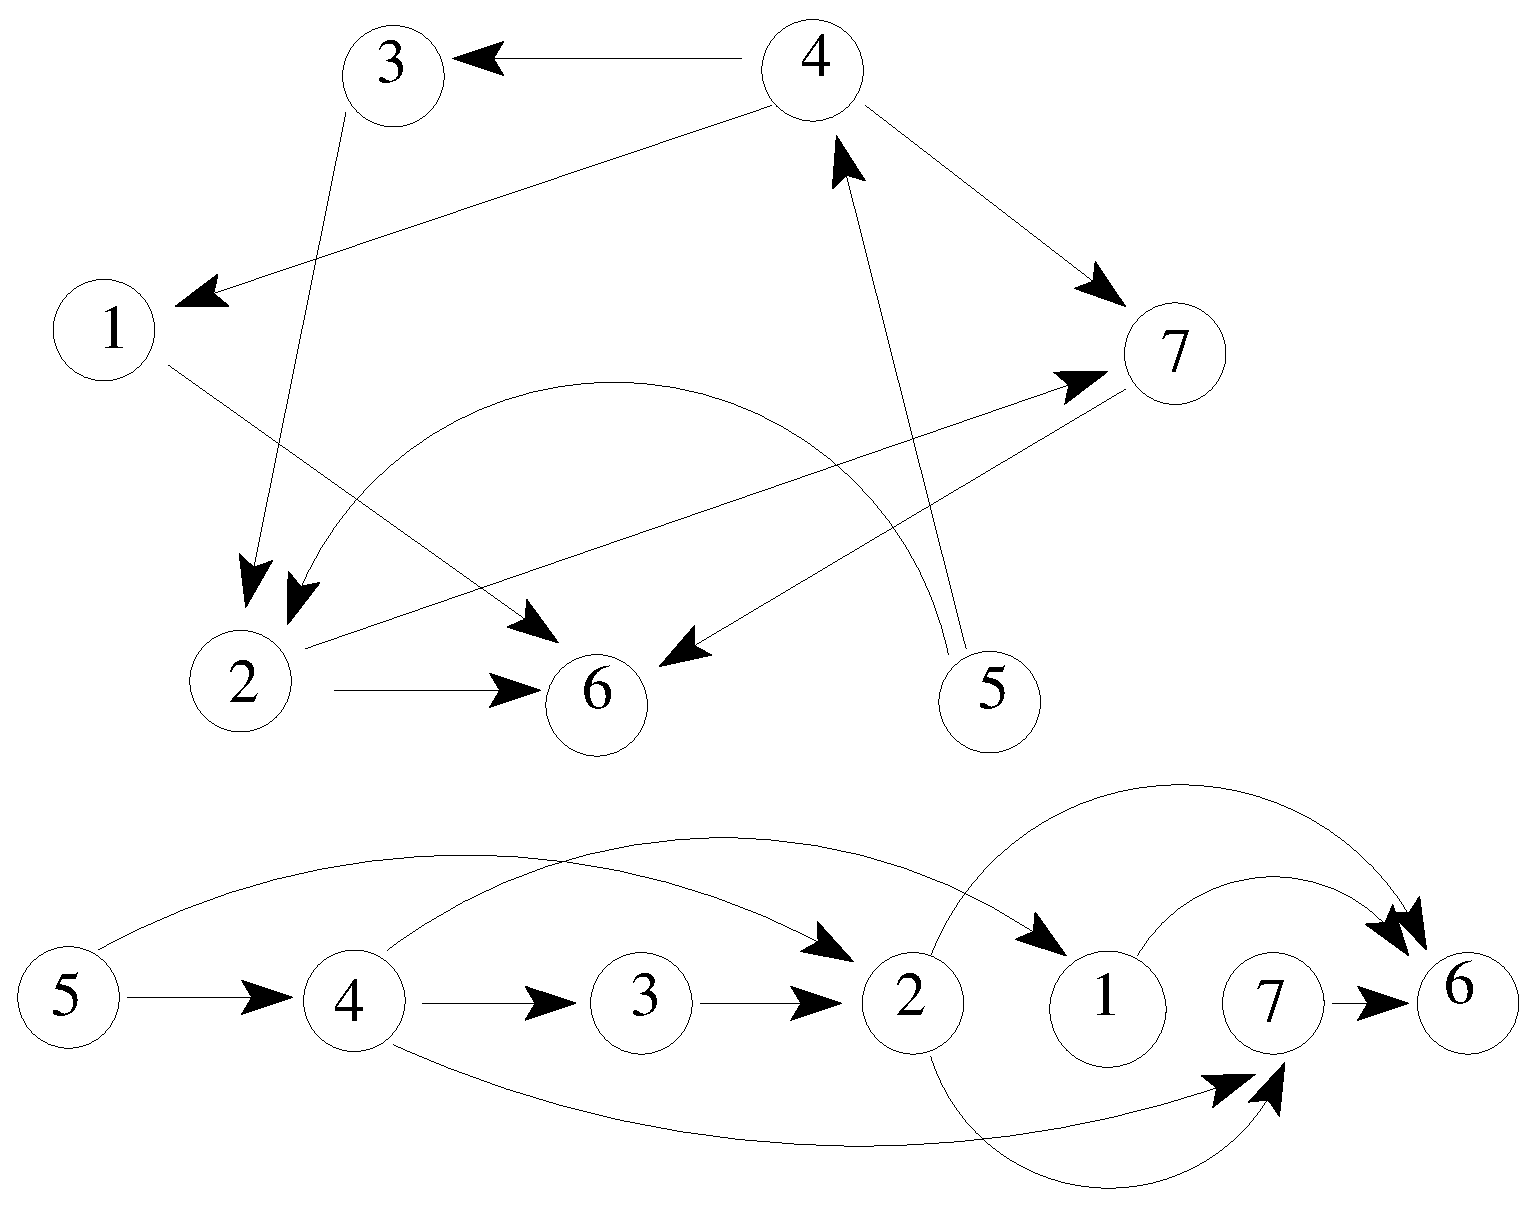
\includegraphics[width=0.6\linewidth]{tritopologique_corrige.eps}
\end{center}


\section{Problème 3~: composantes fortement connexes}
Entourez les composantes fortement connexes.
Dessinez le graphe réduit (chaque sommet du graphe réduit représente une CFC).

\begin{center}
\includegraphics[width=0.55\linewidth]{cfc.eps}
\end{center}

Le sommet 1 qui n'a pas d'arc entrant et  le sommet 6 qui n'a pas d'arc sortant sont réduit à une CFC.
Le sommet 4 n'est accessible que depuis 1, il est donc lui aussi réduit  à une CFC.

Les sommets restants (2, 3, 5) forment une CFC.

Le graphe modifié est donné ci-dessous.

\begin{center}
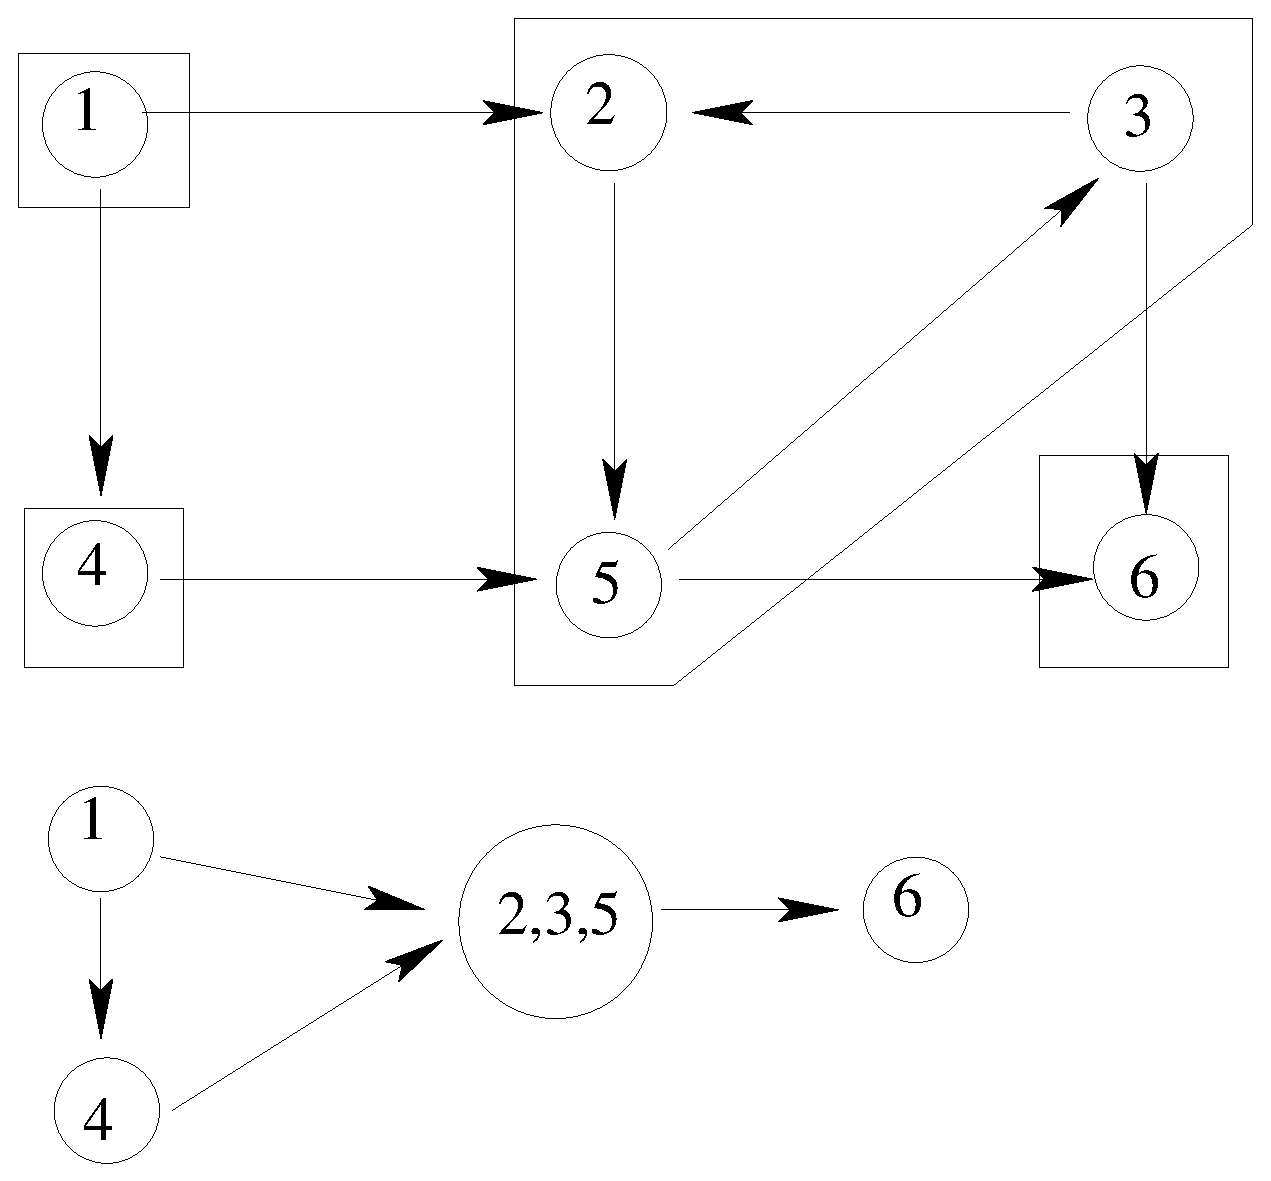
\includegraphics[width=0.5\linewidth]{cfc_bis.eps}
\end{center}


\section{Problème 4~: Euclide et Bézout}
Calculez, avec l'algorithme d'Euclide généralisé, $(x, y, g)$, tels que $g$ soit le PGCD de 72 et 39, 
et que
$72x+39y=g$. 
Donnez le détail de vos calculs (comme en TD), par exemple dans un tableau, ou avec des produits matriciels.

Cet algorithme donne le couple $(x, y)$ tel que
$x^2+y^2$ soit minimal.  
Donnez une formule avec un paramètre $t\in\Z$  permettant de générer toutes les paires  $(x, y)$ telles
que $72x+39y=g$. 

Version 1- tableau calculé avec 1 et 0.

$$\begin{array}{|c|c|c|c|c|c|c|}
\hline
a=72 & b=39 & a\mod b & a\div b & pgcd &u & v \\
\hline
72 & 39 & 33 & 1 & 3 & 6 & -11 \\
 39 & 33  & 6 & 1 & 3 & -5 & 6  \\
33  & 6   & 3 & 5  & 3 & 1 & -5  \\
 6   & 3   & 0 & 2  & 3 & 0     & 1  \\
 3   & 0   &   &    & 3 & 1     & 0  \\
\hline
\end{array}
$$


Version 2- tableau calculé avec 1 et t.

$$\begin{array}{|c|c|c|c|c|c|c|}
\hline
a=72 & b=39 & a\mod b & a\div b & pgcd &u & v \\
\hline
72 & 39 & 33 & 1 & 3 & -13t+6 & 24t-11 \\
 39 & 33  & 6 & 1 & 3 & 11t-5 & -13t+6  \\
33  & 6   & 3 & 5  & 3 & 1-2t & 11t-5  \\
 6   & 3   & 0 & 2  & 3 & t     & 1-2t  \\
 3   & 0   &   &    & 3 & 1     & t  \\
\hline
\end{array}
$$


\section{Problème 5}
Rappel~: Pour calculer efficacement la séquence de Fibonacci, définie par
$F(0)=0, F(1)=1, F(n)= F(n-1)+F(n-2)$, on considère l'expression matricielle~:

\begin{eqnarray*}
 \left( \begin{array}{c} F(n) \\
 F(n-1)
\end{array}\right) &=& 
\left( \begin{array}{cc}  1 & 1 \\
1 & 0
\end{array}\right) \left(\begin{array}{c} F(n-1) \\
 F(n-2)\end{array}\right)   \\
&=& \left( \begin{array}{cc}  1 & 1 \\
1 & 0
\end{array}\right)^{n-1} \left(\begin{array}{c} F(1)\\
F(0)\end{array}\right)
\end{eqnarray*}

Pour calculer rapidement la séquence~: $G(0)=1, G(1)=4, G(n)=2\times G(n-1)+n+1$, quelle expression matricielle faut-il considérer~? Vous pouvez compléter la matrice ci-dessous~:

$$
 \left( \begin{array}{c}
G(n) \\
n\\
1\end{array}\right) = \left( \begin{array}{ccc}
\quad & \quad & \quad \\
\quad & \quad & \quad \\
\quad & \quad & \quad \end{array}\right) \left(\begin{array}{c} G(n-1) \\
n-1\\
1\end{array}\right)
$$

Attention~: la matrice ne doit contenir que des constantes.

La matrice à utiliser est :


$$
 \left( \begin{array}{c}
G(n) \\
n\\
1\end{array}\right) = \left( \begin{array}{ccc}
2 & 1 & 2 \\
0 & 1 & 1 \\
0 & 0 & 1 \end{array}\right) \left(\begin{array}{c} G(n-1) \\
n-1\\
1\end{array}\right)
$$


Expliquez pourquoi cette formulation permet de calculer $F(n)$ ou $G(n)$ rapidement.

Il suffit de calculer la puissance $n$ de la matrice ci-dessus, en utilisant un algorithme de puissance rapide.

En fait, $G(n)=a 2^n +b n + c$. Comment calculeriez-vous
les valeurs des constantes $a, b, c$~?



\section{Quizz}

\begin{enumerate}
\item Citez deux problèmes indécidables en informatique.

La terminaison d’un algorithme (ou d’une
machine de Turing), l’égalité de deux nombres réels (ou complexes), l’égalité de deux fonctions (par
exemple de N dans N).

\item  Quand dit-on qu'un problème, bien que décidable, est difficile en informatique~?

Quand aucun algorithme en temps polynomial permettant de résoudre
ce problème n’est connu.

\item   Citez deux problèmes solubles en informatique, mais difficiles.

Résoudre un problème SAT (où un solveur SAT est un programme qui
décide automatiquement si une formule de logique propositionnelle est
satisfaisable). Trouver un chemin ou un circuit hamiltonie n (passant
par tous les sommets dans un graphe). Trouver une clique max ou un
stable max. Factoriser un très grand entier.

\item   Citez  trois algorithmes efficaces pour trier des nombres, en utilisant des comparaisons. Dire quelle est la complexité de ces algorithmes.

\begin{itemize}
\item tri par fusion  ou mergesort, $O(n  log(n))$
\item tri par tas  ou heapsort, $O(n  log(n))$
\item  tri rapide ou quicksort, en moyenne complexité en $O(n  log(n))$.
\end{itemize}

\item  Citez deux  algorithmes  qui trient des nombres entiers sans effectuer de comparaisons entre les nombres à trier:
\begin{itemize}
\item  le "radix sort", ou tri par base,
\item le tri par comptage lorsque le nombre de valeurs distinctes est faible.
\end{itemize}

\item   Donnez le nom de deux algorithmes calculant les plus courts chemins dans un graphe.
Dijkstra, Floyd, Ford (ou Ford-Bellman), Dantzig,
Warshall, pseudo produit matriciel : (AB) l,c = min k (A lk + B kc ).

\item   Citer trois noms de structures de données vues en cours.

Les listes, piles, files, graphes ... ainsi que les tableaux.

\item Quel est le nom (éventuellement en anglais) de la méthode vue en cours pour résoudre le "problème des reines"~? 

Les algorithmes avec backtrack.
\end{enumerate}
\end{document}
